\documentclass[a1paper,fontscale=0.6]{poster}

\usepackage{graphicx}  % Required for including images
\graphicspath{{figures/}} % Directory in which figures are stored

\usepackage{amsmath}
\usepackage{amssymb}
\usepackage{bm}
\usepackage{enumitem}

\usepackage[font=small,labelfont=bf]{caption}

\definecolor{light}{HTML}{81C4E6} 
\definecolor{medium}{HTML}{3399CC} 
\definecolor{dark}{HTML}{0070A8} 

\begin{document}

\begin{poster}{
headerborder=closed, % Adds a border around the header of content boxes
colspacing=1em, % Column spacing
bgColorOne=white, % Background color for the gradient on the left side of the poster
bgColorTwo=white, % Background color for the gradient on the right side of the poster
borderColor=light, % Border color
headerColorOne=medium, % Background color for the header in the content boxes (left side)
headerColorTwo=medium, % Background color for the header in the content boxes (right side)
headerFontColor=white, % Text color for the header text in the content boxes
boxColorOne=white, % Background color of the content boxes
textborder=rectangle, % Format of the border around content boxes, can be: none, bars, coils, triangles, rectangle, rounded, roundedsmall, roundedright or faded
eyecatcher=true, % Set to false for ignoring the left logo in the title and move the title left
headerheight=0.1\textheight, % Height of the header
headershape=roundedright, % Specify the rounded corner in the content box headers, can be: rectangle, small-rounded, roundedright, roundedleft or rounded
headerfont=\Large\bf\textsc, % Large, bold and sans serif font in the headers of content boxes
%textfont={\setlength{\parindent}{1.5em}}, % Uncomment for paragraph indentation
linewidth=1pt % Width of the border lines around content boxes
}
%----------------------------------------------------------------------------------------
%	TITLE PARAMETERS
%----------------------------------------------------------------------------------------
{
\includegraphics[height=6em]{mmr-text.png}}
{\bf\textsc{numerical modelling of dynamic processes\\\vspace{0.4em} in a nuclear reactor}}
{\vspace{0.4em}
{Aleksandr Vasilev} \\\vspace{0.4em}
\normalsize{
North-Eastern Federal University, Yakutsk \quad
Nuclear Safety Institute, Russian Academy of Sciences, Moscow \quad
haska87@gmail.com}}
{
\includegraphics[height=6em]{logoNEFU.png}}

%----------------------------------------------------------------------------------------
%	INTRODUCTION
%----------------------------------------------------------------------------------------
\headerbox{Introduction}{name=introduction,column=0,row=0}{
The physical processes in a nuclear reactor depend on distribution of neutron flux, whose mathematical description is based on the neutron-transport equation. 
The general view of this equation is integrally-differential one, and the required distribution of neutrons flux depends on time, energy, spatial and angular variables. As a rule, the simplified forms of the neutron transport equation are used for practical calculations of nuclear reactors.
\\

The stationary state of neutron flux, which is related to the critical state of the reactor, is characterised by local balancing of neutron absorption and birth intensities. This boundary state is usually described by solution of a spectral problem ($\lambda$-eigenvalue problem) provided that the fundamental eigenvalue that is called k-effective of the reactor core, is equal to unity. Calculations of k-effective of the reactor on the basis of the spectral Lambda Modes problem solution are obligatory for developing a new design of reactor installation.
}

%----------------------------------------------------------------------------------------
%	Problem statement
%----------------------------------------------------------------------------------------
\headerbox{Problem statement}{name=statement,column=0,below=introduction}{
\textbf{Diffusion approximation}
\[
\frac{1}{v_g}\frac{\partial \phi_g}{\partial t} - \nabla \cdot D_g \nabla \phi_g + \Sigma_{r,g} \phi_g = (1-\beta)\chi_g S_n + S_{s,g} + \tilde{\chi}_g S_d.
\]
\textbf{SP$_3$ approximation}
\[
\begin{split}
 \frac{1}{v_g} \frac{\partial \phi_{0,g}}{\partial t} - \frac{2}{v_g} \frac{\partial \phi_{2,g}}{\partial t} - & \nabla \cdot D_{0,g} \nabla \phi_{0,g} + \Sigma_{r,g} \phi_{0,g} -  2\Sigma_{r,g} \phi_{2,g} = \\ 
 =  & (1-\beta)\chi_{n,g} S_{n} + S_{s,g} + \chi_{d,g} S_d, \\
 -\frac{2}{v_g} \frac{\partial \phi_{0,g}}{\partial t} + \frac{9}{v_g} \frac{\partial \phi_{2,g}}{\partial t} - & \nabla \cdot D_{2,g} \nabla \phi_{2,g} + (5\Sigma_{t,g} + 4\Sigma_{r,g}) \phi_{2,g}  \\ 
- 2\Sigma_{r,g} \phi_{0,g} = & -2(1-\beta)\chi_{n,g} S_{n} - 2S_{s,g} - 2\chi_{d,g} S_d,
\end{split}
\]
where
\[
S_{n} =  \sum_{g'=1}^{G} \nu \Sigma_{f,g'} \phi_{g'}, 
\quad
S_{s,g} = \sum_{g\neq g'=1}^{G} \Sigma_{s,g'\rightarrow g} \phi_{g'},
\quad
S_{d} = \sum_{m=1}^{M} \lambda_m c_m,
\]
\[
\phi_{0,g}=\phi_g + 2\phi_{2,g}, 
\quad
D_{0,g} = \cfrac{1}{3\Sigma_{tr,g}}, 
\quad
D_{2,g} = \cfrac{9}{7\Sigma_{t,g}}, 
\quad g=1,2,...,G.
\]
\textbf{Delayed neutrons source}
\[
 \frac{\partial c_m}{\partial t} + \lambda_m c_m = \beta_m S_{n},
 \quad \beta = \sum_{m=1}^{M} \beta_m,
 \quad m = 1,2, ..., M.
\]
Here $G$ -- number of energy groups,
$M$ -- number of types of delayed neutrons,
$\phi_g(\bm x, t)$ -- scalar flux,
$\phi_{0,g}(\bm x, t)$ -- 0th moment of angular flux,
$\phi_{2,g}(\bm x, t)$ -- 2th moment of angular flux,
$c_m(\bm x, t)$ -- density of sources of delayed neutrons.
\\

\textbf{Boundary condition}

The Albedo-type conditions (for diffusion approximation)
\[
D_g \frac{\partial\phi_g}{\partial n} + \gamma_g \phi_g = 0,
\]
where $n$ is outter normal to the boundary.


The Marshak-type conditions (for SP$_3$ approximation) $i = 0, 2$
\[
\begin{split}
\begin{bmatrix}
J_{0,g}(\bm x)\\
J_{2,g}(\bm x)\\
\end{bmatrix}
=
\begin{bmatrix}
\phantom{-}\cfrac{1}{2} & -\cfrac{3}{8} \\
 -\cfrac{3}{8} & \phantom{-}\cfrac{21}{8} \\
\end{bmatrix}
\begin{bmatrix}
\phi_{0,g}(\bm x) \\
\phi_{2,g}(\bm x) \\
\end{bmatrix},
\quad
J_{i,g}(\bm x) = -D_{i,g}\nabla\phi_{i,g}(\bm x).
\end{split}
\]
The \textbf{Cauchy problem} is formulated when
\[
 \bm u_1(0) = \bm u_1^0, \quad  \bm u_2(0) = \bm u_2^0, \quad \bm c(0) = \bm c^0,
\]
where $\bm u_1^0 = \{\phi_{0,1}^0,  \phi_{0,2}^0, ...,  \phi_{0,G}^0 \}$, 
$\bm u_2^0 = \{\phi_{2,1}^0,  \phi_{2,2}^0, ...,  \phi_{2,G}^0 \}$ and \\
$\bm c^0 = \{ c_1^0,  c_2^0, ...,  c_M^0 \}$.

}

\headerbox{Spectral problems}{name=spectral,column=0,below=statement}{
To characterize the reactor dynamic processes described by Cauchy problem, let's consider some spectral problems.
The spectral problem, which is known as the \textbf{$\lambda$-spectral problem}, is usually considered
\[
L \bm \varphi = \lambda^{(k)} M \bm \varphi,
\]
where
\[
\bm \varphi = \{\bm \varphi_1, \bm \varphi_2\},
\quad
L = \begin{pmatrix}
A_1 & B \\
B & A_2 \\
\end{pmatrix},
\quad
M = \begin{pmatrix}
F & -2F \\
-2F & 4F \\
\end{pmatrix}.
\]
The minimal eigenvalue is used for characterisation of neutron field, thus
$
 k = \frac{1}{\lambda^{(k)}_1}  
$
is the effective multiplication factor (k-effective).

\vspace{0.5em}
The $\lambda$-spectral problem cannot directly be connected with the
dynamic processes in a nuclear reactor. The more acceptable spectral characteristics for the non-stationary equation are related the \textbf{$\alpha$-spectral problem}
\[
\begin{split}
L \bm \varphi - (1 - \beta) M \bm \varphi - I \bm s &= \lambda^{(\alpha)} W \bm \varphi, \\
\Lambda \bm s - R \bm \varphi  &= \lambda^{(\alpha)} \bm s.
\end{split}
\]
where
\[
I = \begin{pmatrix}
E \\
-2E \\
\end{pmatrix},
\quad
R = \begin{pmatrix}
Q & -2Q \\
\end{pmatrix},
\quad
W = \begin{pmatrix}
V & -2V \\
-2V & 9V \\
\end{pmatrix}
\]
The fundamental eigenvalue
$
 \alpha = \lambda^{(\alpha)}_1
$
is called the $\alpha$-eigenvalue or the period eigenvalue, because it is inversely related to the reactor period.

To study the properties of the eigenvalues and eigenfunctions of dufferent types, several benchmarks are studied (Fig 1 and 2).
}

\headerbox{}{name=spectral2,column=1}{
\begin{minipage}{0.5\textwidth}
\begin{center}
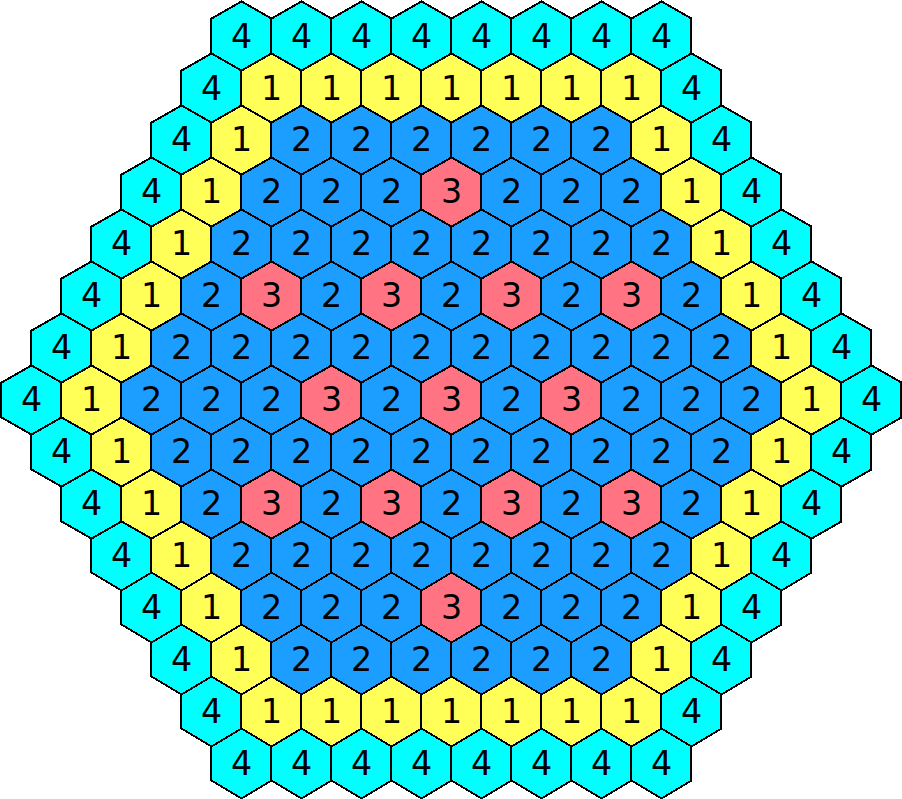
\includegraphics[width=0.7\linewidth]{spectral/iaea_reflector.png}\\
\vspace{-0em}
\footnotesize{Fig.1. IAEA geometry}
\end{center}
\end{minipage}
\begin{minipage}{0.5\textwidth}
\begin{center}
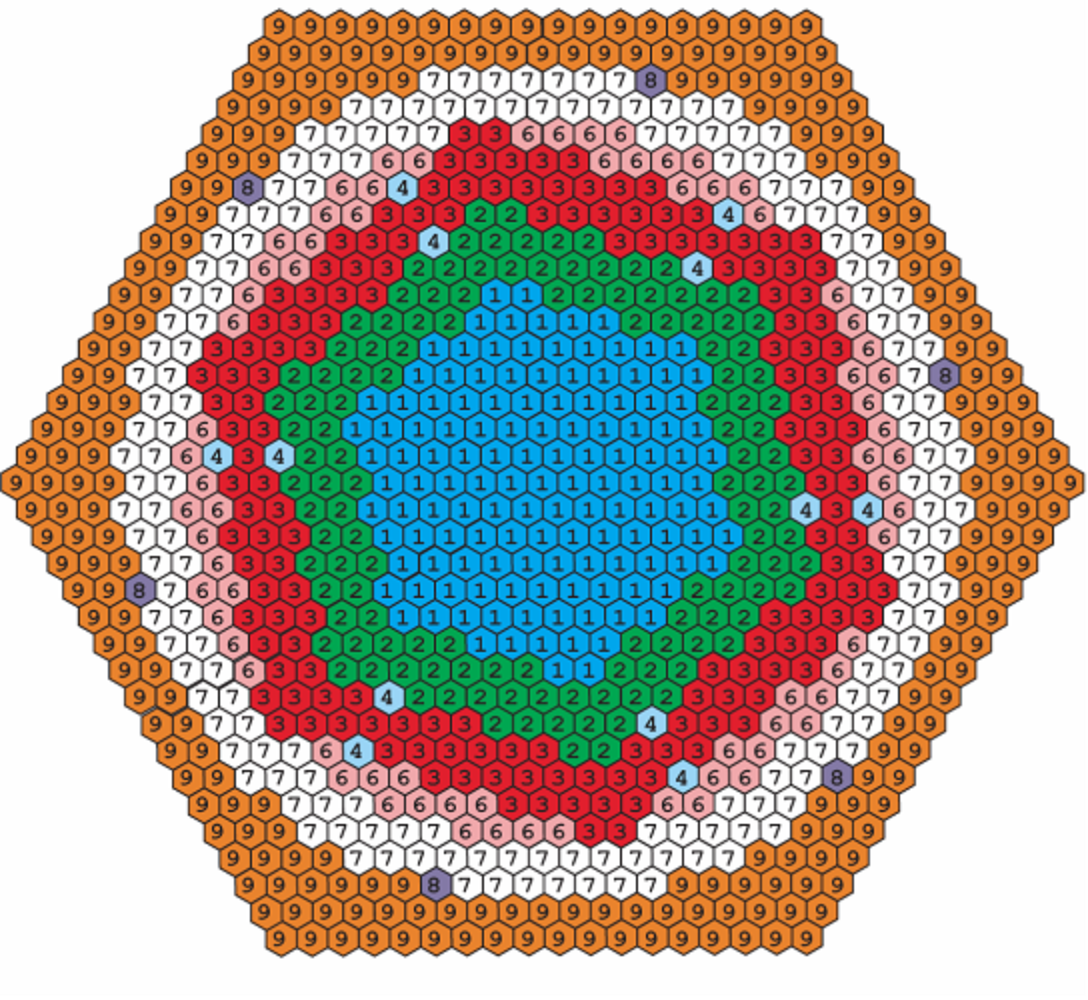
\includegraphics[width=0.7\linewidth]{spectral/hwr.png}\\
\vspace{-0.5em}
\footnotesize{Fig.2. HWR geometry}
\end{center}
\end{minipage}

\vspace{0.5em}
The results of the solution of $\lambda$-spectal problem are shown in Fig. 3, 4. 
(blue -- diffusion model, green -- SP$_3$ model)

\begin{minipage}{0.5\textwidth}
\begin{center}
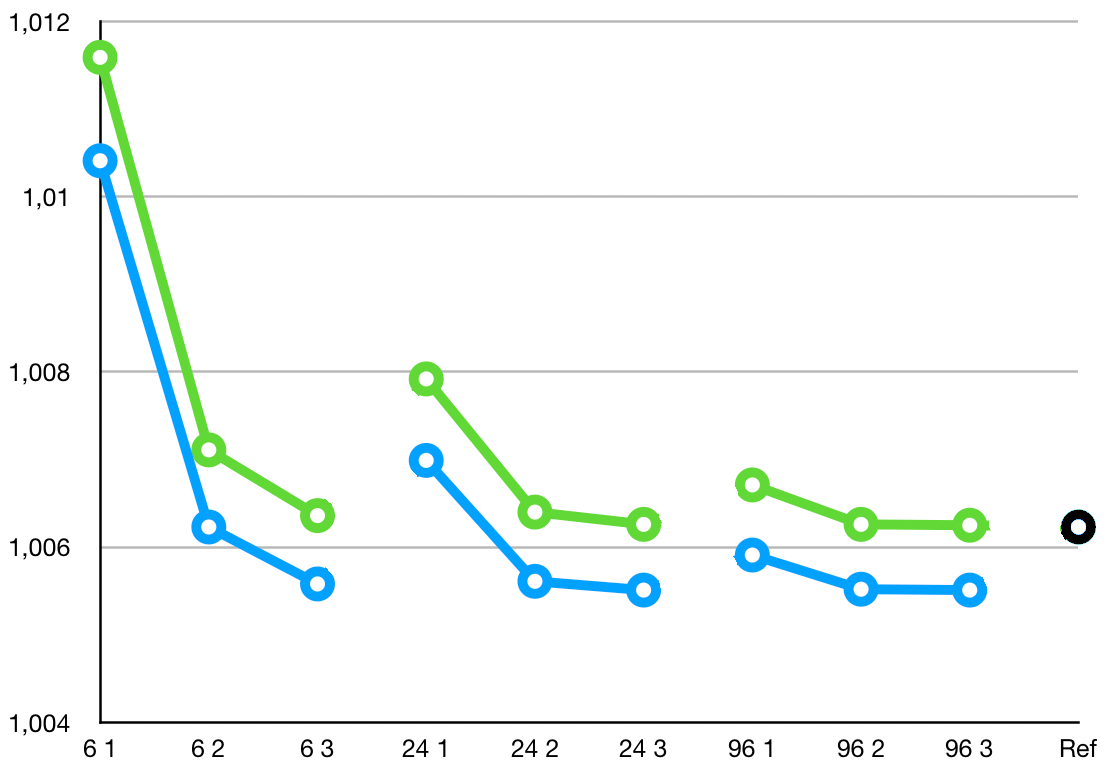
\includegraphics[width=0.7\linewidth]{spectral/iaea_k.png}\\
\vspace{-0em}
\footnotesize{Fig.3. $k$ for IAEA}
\end{center}
\end{minipage}
\begin{minipage}{0.5\textwidth}
\begin{center}
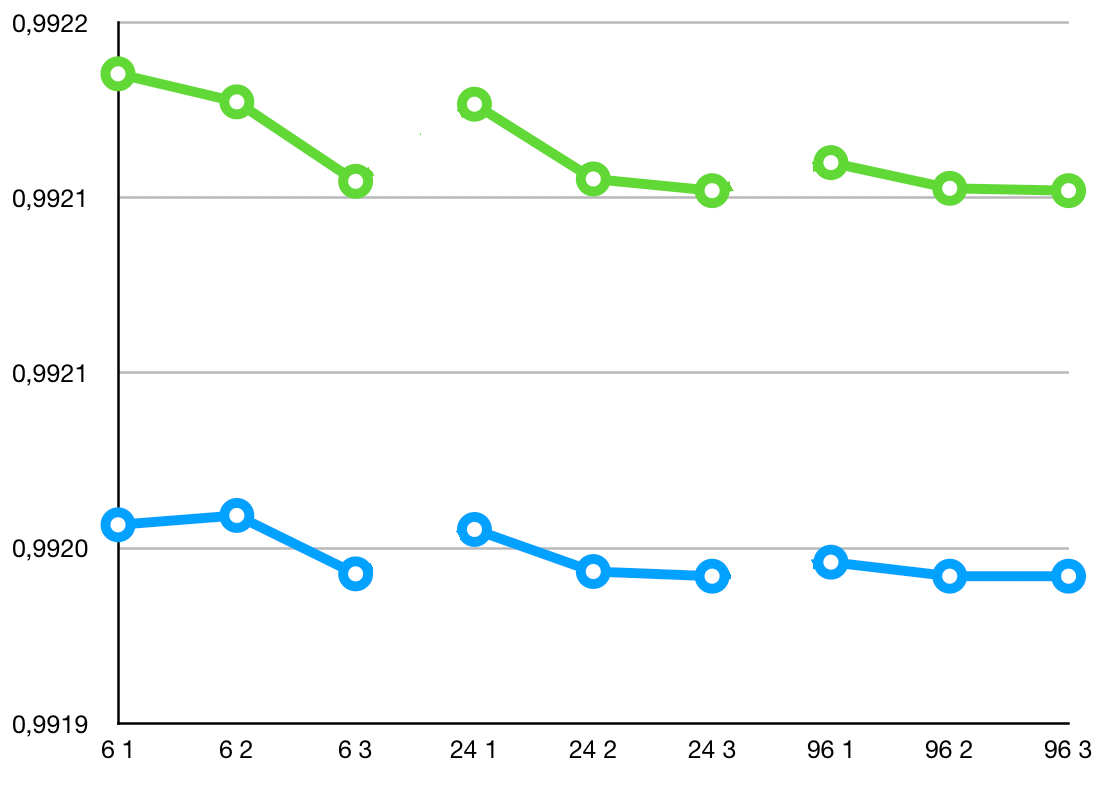
\includegraphics[width=0.7\linewidth]{spectral/hwr_k.png}\\
\vspace{-0.5em}
\footnotesize{Fig.4. $k$ for HWR}
\end{center}
\end{minipage}

\vspace{0.5em}
The $\alpha$-spectral problem with delayed neutrons results for the first 10 eigenvalues are shown in table below: left -- IAEA, right -- HWR.

\begin{minipage}{0.5\textwidth}
\begin{center}
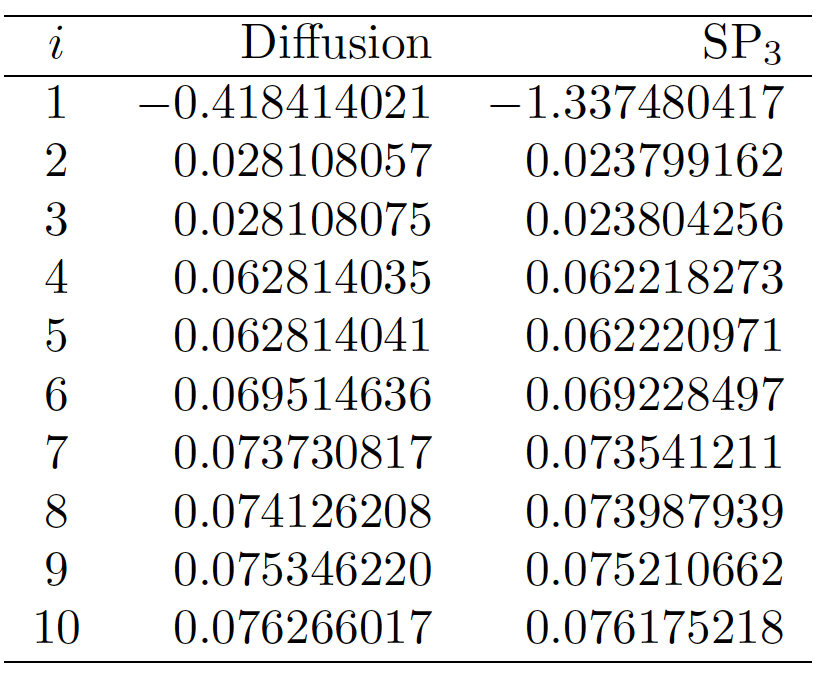
\includegraphics[width=0.7\linewidth]{spectral/iaea2d_alpha_10.png}\\
\end{center}
\end{minipage}
\begin{minipage}{0.5\textwidth}
\begin{center}
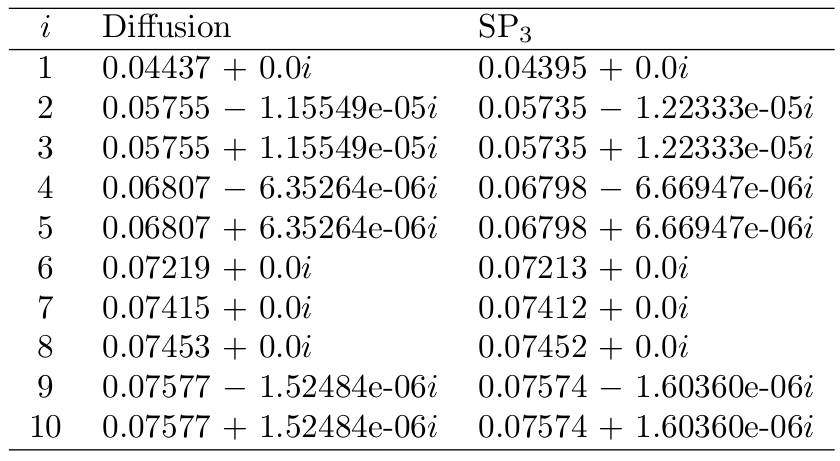
\includegraphics[width=1\linewidth]{spectral/hwr_alpha_del_10.png}\\
\end{center}
\end{minipage}

Of particular interest is the problem associated with appearance of complex eigenvalues and eigenfunctions. 
It was found that this tendency occurs for both the diffusion and $\mathrm{SP_3}$ solutions of the HWR reactor test. 

\begin{center}
\begin{minipage}{0.051\linewidth}
\end{minipage}
\begin{minipage}{0.25\linewidth}
\center{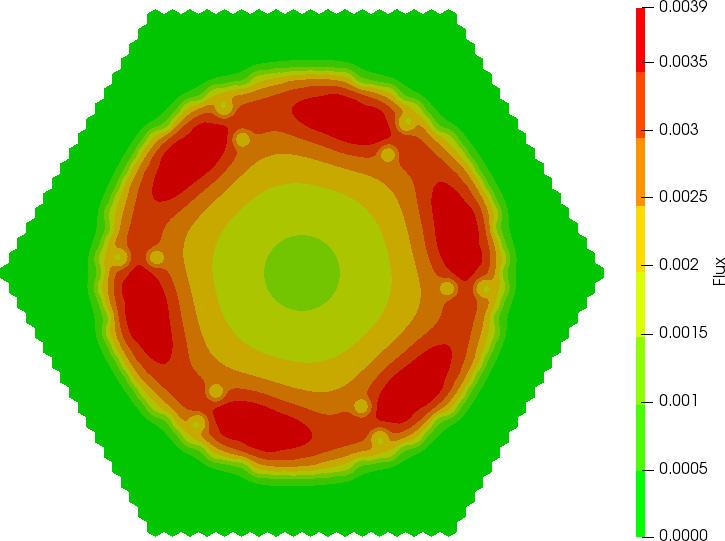
\includegraphics[width=1\linewidth]{hwr/alpha_delayed_sp3_rx1_1.png}} \\
\end{minipage}
\hfill
\begin{minipage}{0.25\linewidth}
\center{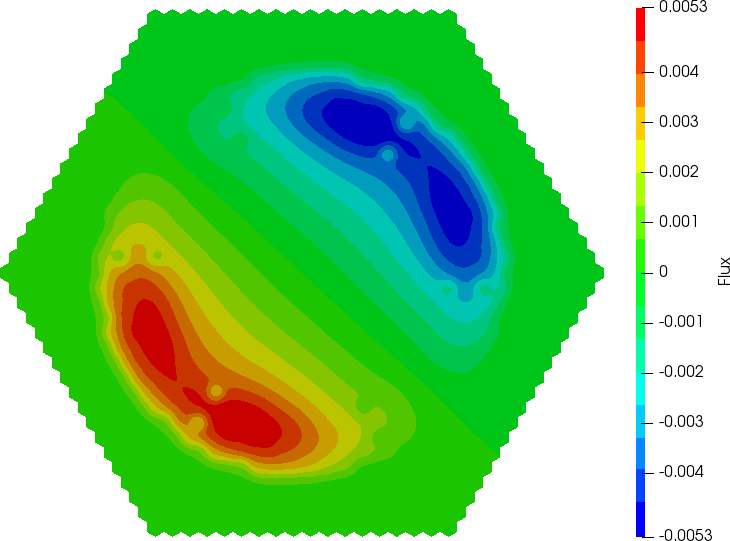
\includegraphics[width=1\linewidth]{hwr/alpha_delayed_sp3_rx1_2}} \\
\end{minipage}
\hfill
\begin{minipage}{0.25\linewidth}
\center{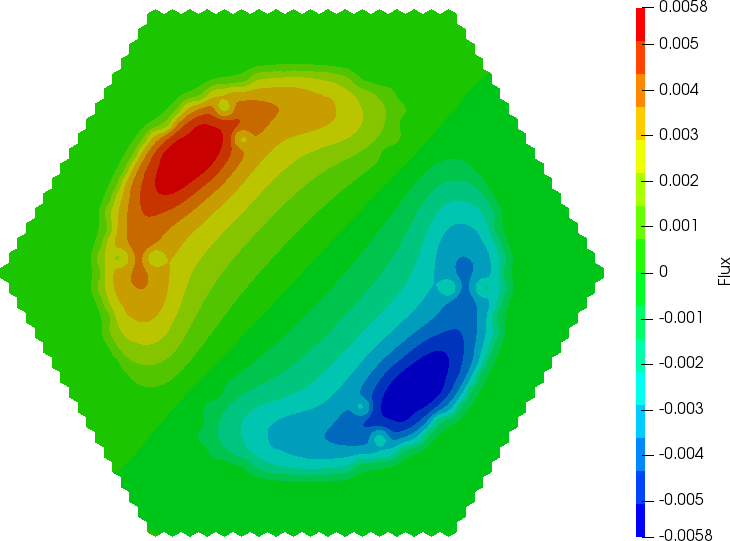
\includegraphics[width=1\linewidth]{hwr/alpha_delayed_sp3_cx1_2}} \\
\end{minipage}

\begin{minipage}{0.051\linewidth}
\end{minipage}
\begin{minipage}{0.25\linewidth}
\center{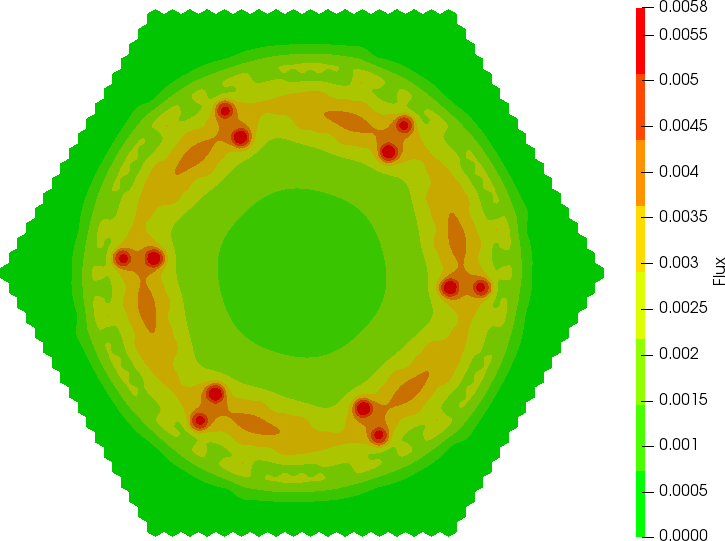
\includegraphics[width=1\linewidth]{hwr/alpha_delayed_sp3_rx2_1.png}} \\
\end{minipage}
\hfill
\begin{minipage}{0.25\linewidth}
\center{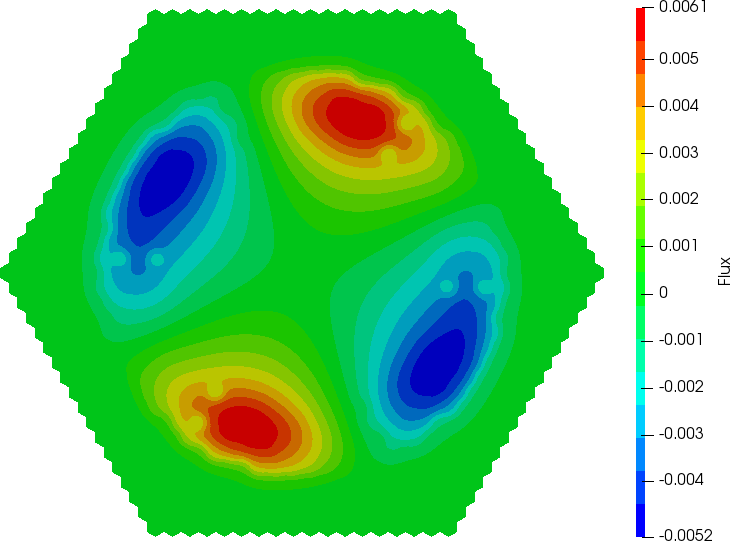
\includegraphics[width=1\linewidth]{hwr/alpha_delayed_sp3_rx1_4}} \\
\end{minipage}
\hfill
\begin{minipage}{0.25\linewidth}
\center{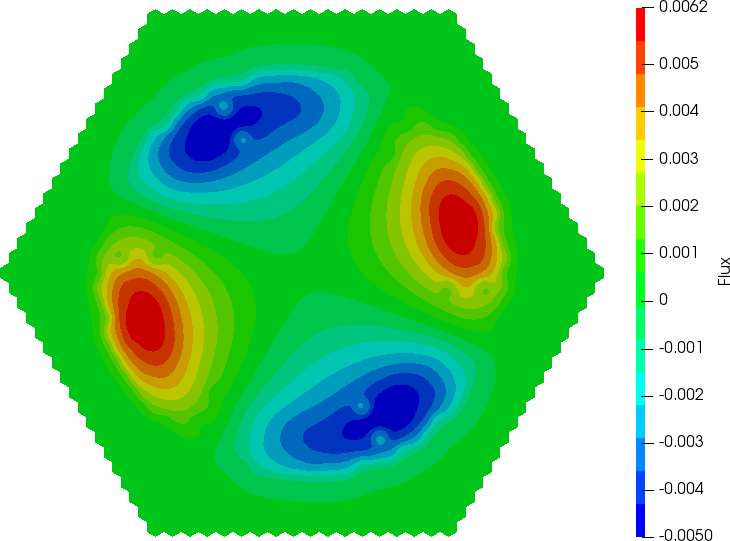
\includegraphics[width=1\linewidth]{hwr/alpha_delayed_sp3_cx1_4}} \\
\end{minipage}

\begin{minipage}{0.051\linewidth}
\end{minipage}
\hfill
\begin{minipage}{0.25\linewidth}
\hspace{0.75em} a \\
\end{minipage}
\hfill
\begin{minipage}{0.25\linewidth} 
\hspace{1.5em} b \\
\end{minipage}
\hfill
\begin{minipage}{0.25\linewidth}
\hspace{2.75em} c \\
\end{minipage}
\\
\vspace{-1em}
\footnotesize{Fig.5. Eigenfunctions: a -- fundamental eigenfunctions; b -- real part of $\phi_1^{(2)}$,$\phi_1^{(3)}$ and $\phi_1^{(4)}$,$\phi_1^{(5)}$; c -- imaginary parts of $\phi_1^{(2)}$,$-\phi_1^{(3)}$ and $\phi_1^{(4)}$,$-\phi_1^{(5)}$.}
\end{center}

The eigenfunctions for fundamental eigenvalue and the real and imaginary part of the eigenfunctions $\phi^{(n)}_1, \ n = 2,3,4,5$ of the $\alpha$-spectral problem  are shown in Fig. 5. The eigenfunctions of the $\lambda$-spectral and $\alpha$-spectral problems are close to each other in topology.

}

\headerbox{Automatic Time Step Selection}{name=timestep,column=1, below=spectral2}{
The main approach is that  the error of the approximate solution is estimated at a new time step on the basis of additional calculations.
The step is estimated from the theoretical asymptotic dependence of the accuracy on time step and after that correction of step is applied, if necessary, the calculations are repeated.
\\

\textbf{Time step selection algorithm}
\begin{center}
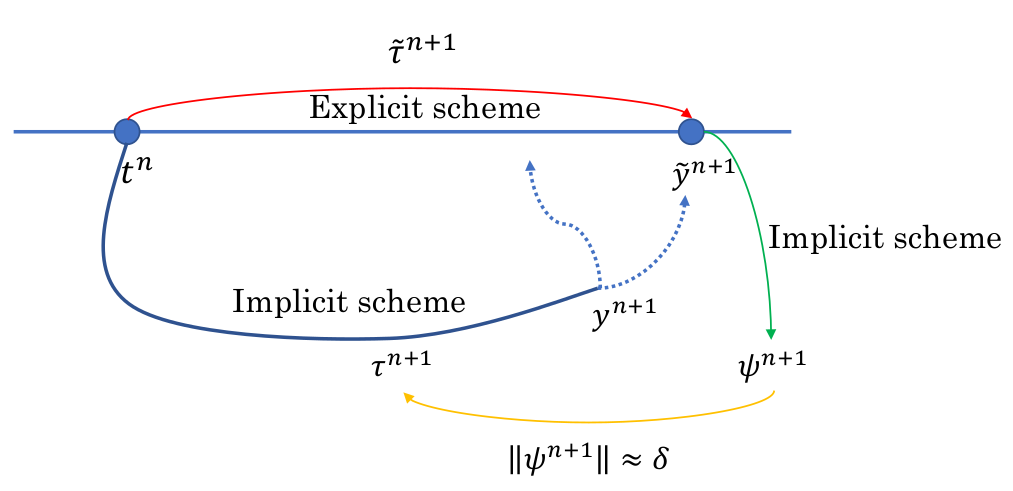
\includegraphics[width=0.8\linewidth]{timestep/algorithm.png}
\end{center}

\begin{enumerate}[noitemsep]
\item 
Predictable time step: $\widetilde{\tau}^{n+1} = \gamma \tau^n$ (eg $\gamma=1.25$)
\item Predictive solution $\widetilde{y}^{n+1}$: an explicit scheme, $\widetilde{t}^{n+1} = t^n + \widetilde{\tau}^{n+1}$
\item Estimation of approximation error: by found $\widetilde{y}^{n+1}$ from an implicit scheme
\item Step selection $\tau^{n+1}$: $\ \|\psi^{n+1}\| \approx \delta$
\item Solution on a new time layer $y^{n+1}$: an implicit scheme, $t^{n+1}=t^n + \tau^{n+1}$
\end{enumerate}

The needed time step $\tau^{n+1} = \max \big \{\tau^0, \min \{\gamma_{n+1}, \gamma \} \tau^n \big \}$, where
\[
  \gamma_{n+1} = \frac{\delta}{ \| (A^{n+1} - A^n) \bm{\varphi^n}  +
  A^{n+1} (\bm{\widetilde{\varphi}^{n+1}} - \bm{\varphi^n}) \| } \gamma. 
\]
This formula clearly shows the corrective actions which are associated with the problem operator and with the dynamics of the
solution.

\begin{center}

\begin{minipage}{0.051\linewidth}
\end{minipage}
\begin{minipage}{0.3\linewidth}
\center{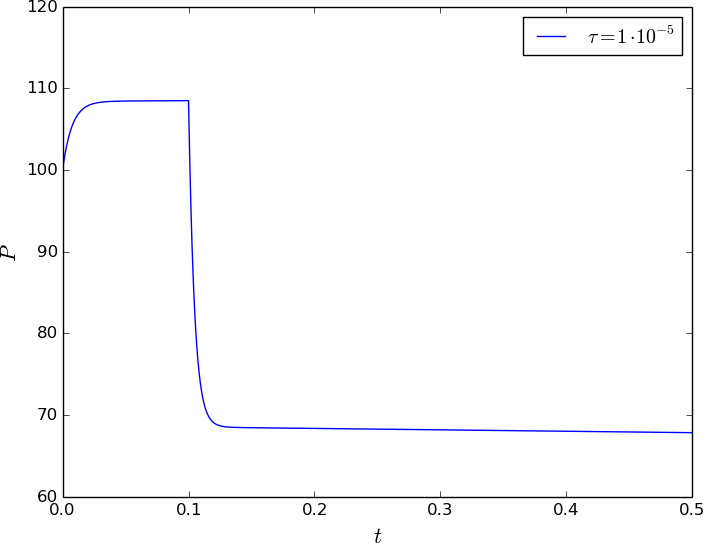
\includegraphics[width=1\linewidth]{timestep/power_down.png}} \\
\end{minipage}
\hfill
\begin{minipage}{0.3\linewidth}
\center{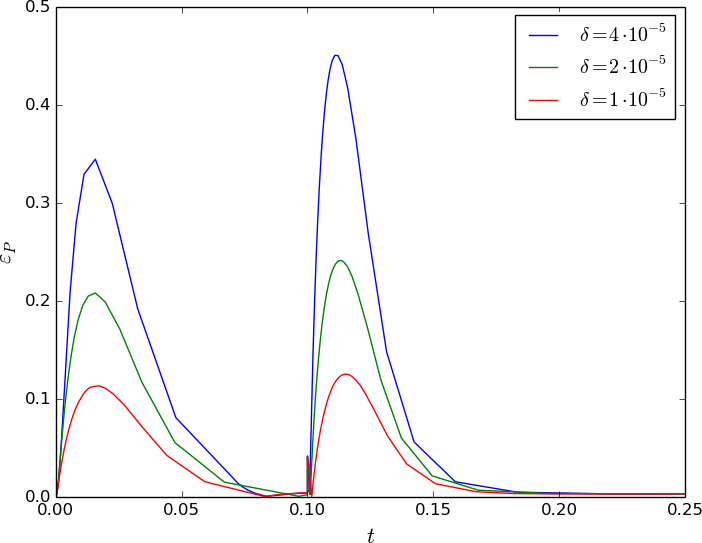
\includegraphics[width=1\linewidth]{timestep/delta_down.png}} \\
\end{minipage}
\hfill
\begin{minipage}{0.3\linewidth}
\center{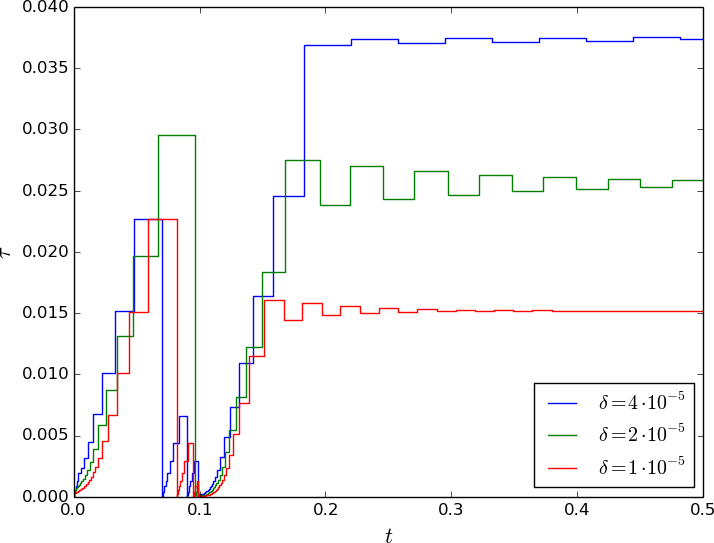
\includegraphics[width=1\linewidth]{timestep/step_down.png}} \\
\end{minipage}

\begin{minipage}{0.051\linewidth}
\end{minipage}
\hfill
\begin{minipage}{0.25\linewidth}
\hspace{2em} a \\
\end{minipage}
\hfill
\begin{minipage}{0.25\linewidth}
\hspace{2em} b \\
\end{minipage}
\hfill
\begin{minipage}{0.25\linewidth}
\hspace{3em} c \\
\end{minipage}
\\
\vspace{-1em}
\footnotesize{Fig.6. a -- power 1, b -- error ($\epsilon_P$), c -- time steps ($n$).}
\end{center}

\begin{center}
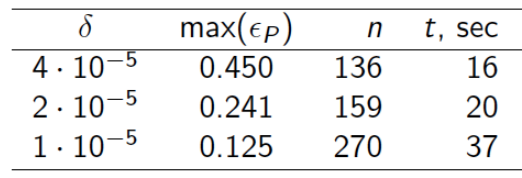
\includegraphics[width=0.5\linewidth]{timestep/table.png}
\end{center}
\vspace{-1em}
Reference solution: fixed time step is 10$^{-5}$, number of steps is 50000,
counting time is 2130 sec.
}

\headerbox{State change modal method}{name=scmm,column=2,row=0}{
The state of the reactor is characterized by the constant coefficients of the system of multigroup diffusion equations.
\begin{center}
    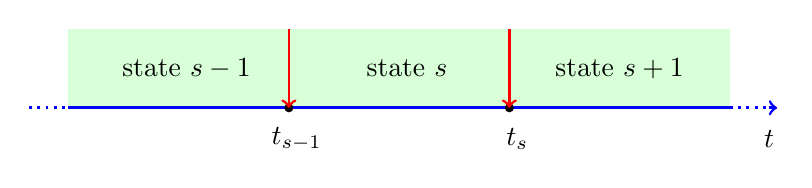
\begin{tikzpicture}
      \filldraw [color=green!15] (-0.5,0) rectangle +(8.4,1);
      \draw [dotted, line width=1, color=blue] (-1,0) -- (-0.5,0);
      \draw [line width=1, color=blue] (-0.5,0) -- (7.9,0);
      \draw [dotted, line width=1, color=blue] (7.9,0) -- (8.4,0);
      \draw [->, line width=1, color=blue] (8.4,0) -- (8.5, 0);
      \filldraw [black] (2.3,0) circle (0.05);
      \filldraw [black] (5.1,0) circle (0.05);
      \draw  (1.0,0.5) node {state $s-1$};  
      \draw  (3.8,0.5) node {state $s$};  
      \draw  (6.5,0.5) node {state $s+1$};  
      \draw  (2.4,-0.4) node {$t_{s-1}$}; 
      \draw  (5.2,-0.4) node {$t_{s}$}; 
      \draw  (8.4,-0.4) node {$t$}; 
      \draw [->, line width=1, color=red] (2.3,1) -- (2.3,0);
      \draw [->, line width=1, color=red] (5.1,1) -- (5.1,0);
    \end{tikzpicture}
\end{center}

%Dynamic processes in a nuclear reactor can be considered as a change of states. 
At a certain time $t = t_s, \ s = 1,2, ...$ an instantaneous change of state occurs. 
The state $s$ is defined by the parameters in equations.
Dynamic behaviour of these components is due to different time-scale processes. 
\vspace{1em}

Delayed neutrons source determines \textbf{slow processes}, when  $\bm c(\bm x,t)$ changes slightly with the reactor state change. In contrast, neutron flux $\bm \phi(\bm x,t)$ determines \textbf{fast processes} when the reactor state changes. 

\begin{description}
\item[Off-line calculation.] 
Calculation of the coefficients for the isolated reactor states, which is performed in advance. 
The status passport also includes calculated dominant eigenvalues and eigenfunctions of the  $\alpha$-eigenvalue problem. 
\item[On-line calculation.]
Real-time modeling is carried out on the basis of the modal solution of the problem.
The coefficients in the representation are calculated from the initial condition. 
The solution for other time intervals is determined according to modal approximation.   
\end{description} 

The dynamics of the 2D VVER-1000 (Fig. 7) reactor during the transition from the supercritical mode to the subcritical mode

\begin{minipage}{0.3\textwidth}
\begin{center}
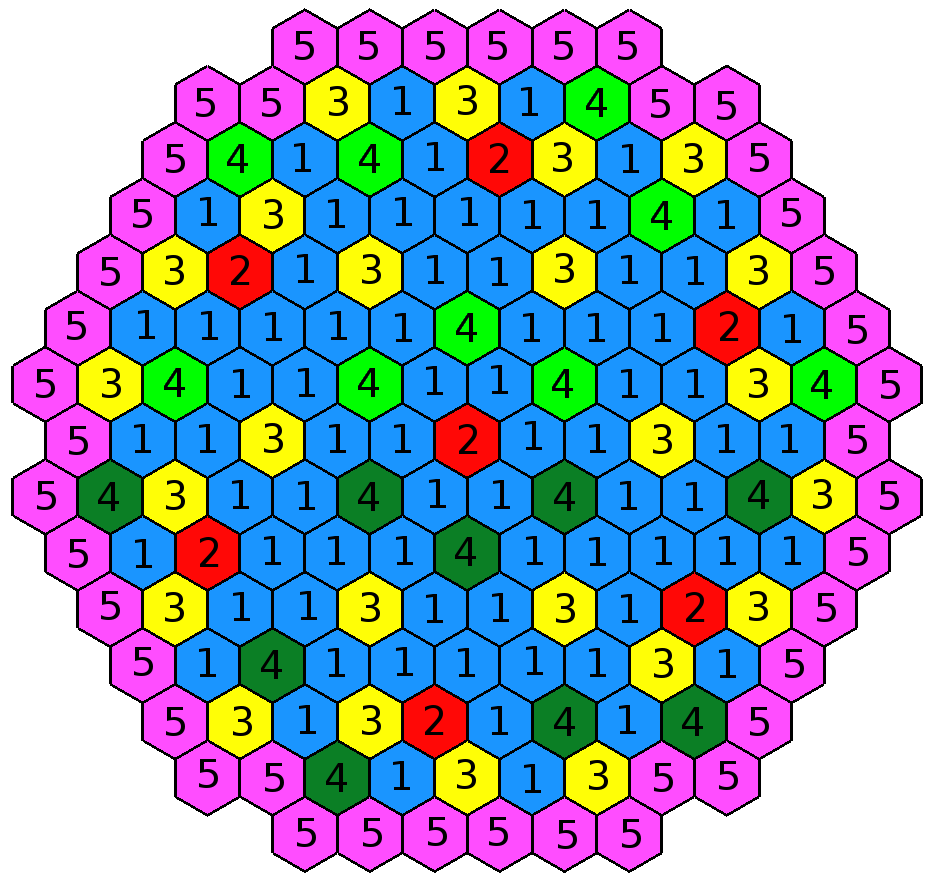
\includegraphics[width=0.8\linewidth]{scmm/geo.png}\\
\footnotesize{Fig.7. VVER-1000}
\end{center}
\end{minipage}
\begin{minipage}{0.7\textwidth}
\begin{itemize}
\setlength\itemsep{0em}
\item 2 group prompt and 1 group of delayed neutrons
\item $\kappa$: from 6 to 96, $p$: from 1 to 3
\item 2 types of perturbation
\end{itemize}
\end{minipage}

\vspace{0.5em}
The coefficients $b_n, \ n = 1,2, ..., N$, $N=50$ of the approximate solution with the initial condition are shown in Fig. 8 (top).

\begin{minipage}{0.5\textwidth}
\begin{center}
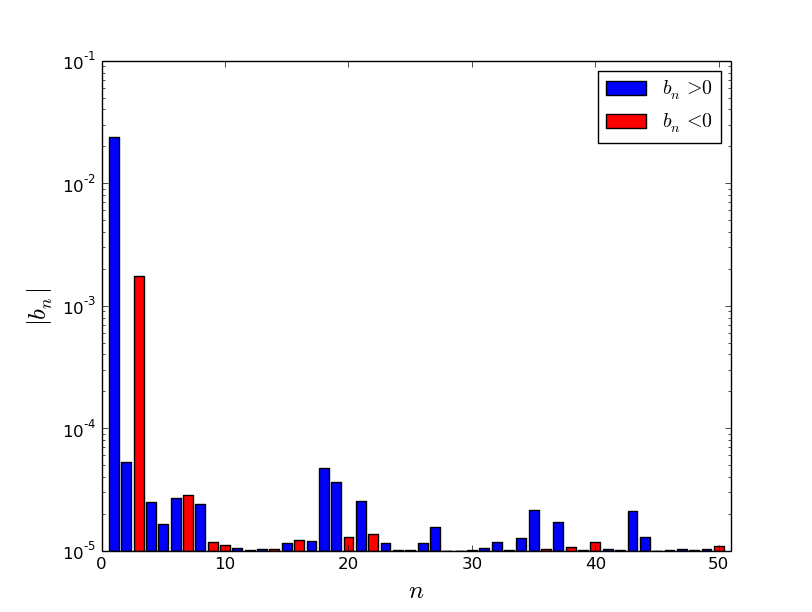
\includegraphics[width=0.75\linewidth]{scmm/12.png}
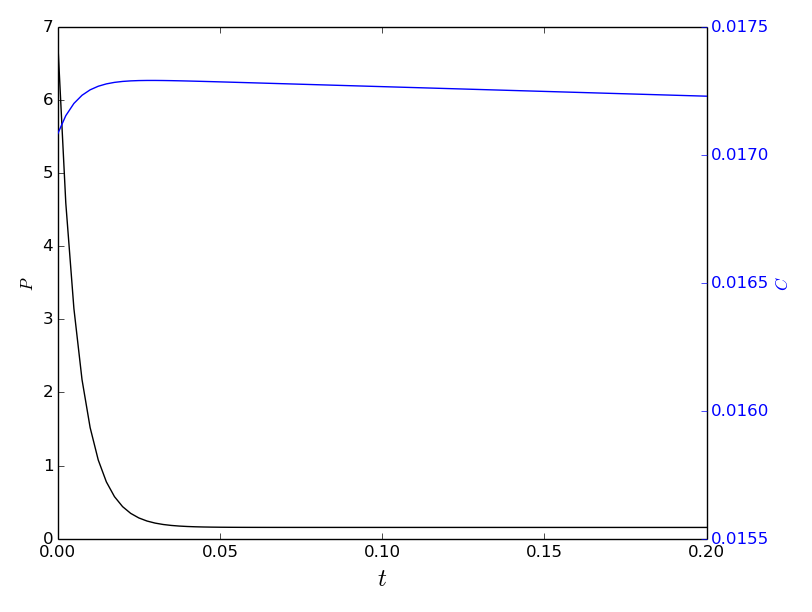
\includegraphics[width=0.75\linewidth]{scmm/14.png}\\
\vspace{-0.5em}
\footnotesize{Fig.8. Coefficients and power}
\end{center}
\end{minipage}
\begin{minipage}{0.5\textwidth}
\begin{center}
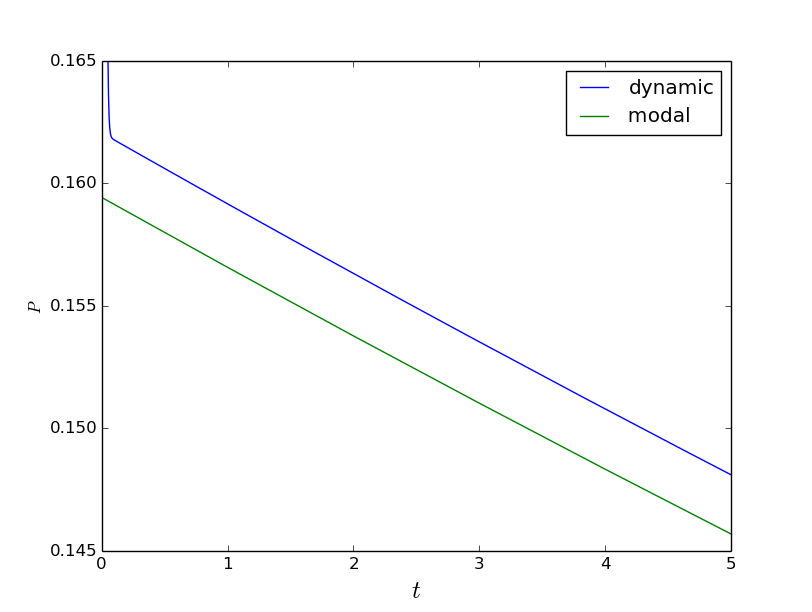
\includegraphics[width=0.75\linewidth]{scmm/17.png}
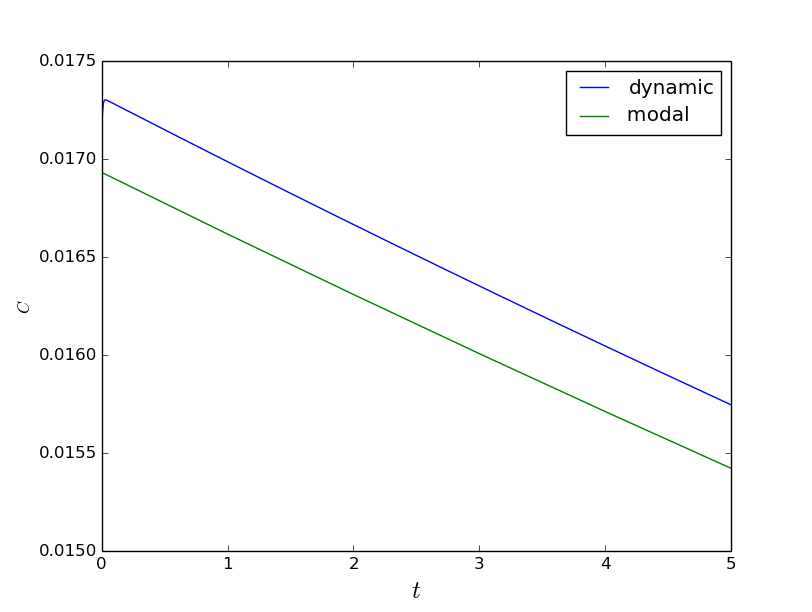
\includegraphics[width=0.75\linewidth]{scmm/18.png}\\
\vspace{-0.5em}
\footnotesize{Fig.9. Neutronic power and delayed neutrons sourse}
\end{center}
\end{minipage}

\vspace{0.5em}
The dynamics of the neutron power of the nuclear reactor and the delayed neutrons source at the initial stage during the transition from the critical state to the subcritical is shown in Fig. 8 (bottom). 

\vspace{0.5em}
The dynamics of the slow phase is illustrated in Figs. 9.
\begin{center}
\begin{minipage}{0.051\linewidth}
\center{1} \\
\end{minipage}
\hfill
\begin{minipage}{0.25\linewidth}
\center{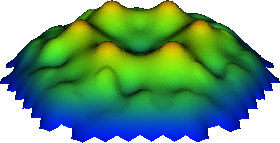
\includegraphics[width=1\linewidth]{scmm/13-11.png}} \\
\end{minipage}
\hfill
\begin{minipage}{0.25\linewidth}
\center{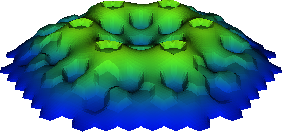
\includegraphics[width=1\linewidth]{scmm/13-12.png}} \\
\end{minipage}
\hfill
\begin{minipage}{0.25\linewidth}
\center{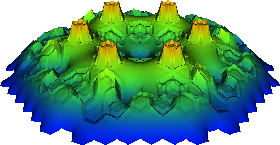
\includegraphics[width=1\linewidth]{scmm/13-13.png}} \\
\end{minipage}

\begin{minipage}{0.051\linewidth}
\center{2} \\
\end{minipage}
\hfill
\begin{minipage}{0.25\linewidth}
\center{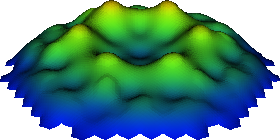
\includegraphics[width=1\linewidth]{scmm/13-21.png}} \\
\end{minipage}
\hfill
\begin{minipage}{0.25\linewidth}
\center{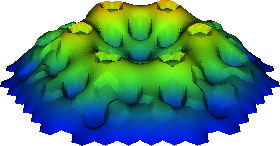
\includegraphics[width=1\linewidth]{scmm/13-22.png}} \\
\end{minipage}
\hfill
\begin{minipage}{0.25\linewidth}
\center{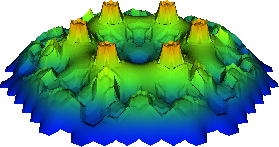
\includegraphics[width=1\linewidth]{scmm/13-23.png}} \\
\end{minipage}

\begin{minipage}{0.051\linewidth}
\center{~} \\
\end{minipage}
\hfill
\begin{minipage}{0.25\linewidth}
\center{a} \\
\end{minipage}
\hfill
\begin{minipage}{0.25\linewidth}
\center{b} \\
\end{minipage}
\hfill
\begin{minipage}{0.25\linewidth}
\center{c} \\
\end{minipage}
\hfill
\\
\footnotesize{Fig.10. Function $\bm u(\bm x, 0)$ (string 1) and function  $\bm u_N(\bm x, 0)$ (string 2): a -- neutron flux of group 1, b -- neutron flux of group 2, c -- delayed neutrons source.}
\end{center}
The beginning and the end of the fast phase are illustrated through the
calculational data shown in Fig. 10.
}

\headerbox{Publications}{name=publication,column=2,below=scmm}{

\begin{enumerate}%[noitemsep]
\item Avvakumov A.~V., et.~al. \textit{State change modal method for numerical simulation of dynamic processes in a nuclear reactor} // Progress in Nuclear Energy. -- 2018. -- Vol. 108. -- P. 240-261.
\item Avvakumov A.~V., et.~al. \textit{Modelling dynamic processes in a nuclear reactor by state change modal method} // Journal of Physics: Conference Series. -- IOP Publishing, 2017. --V. 937. -- No 1. -- P. 012003.
\item Avvakumov A.~V., et.~al. \textit{Automatic Time Step Selection for Numerical Solution of Neutron Diffusion Problems} //International Conference on Finite Difference Methods. -- Springer, Cham, 2018. -- P. 145-152.
\item Vabishchevich P.~N., Vasil\' ev A.~O. \textit{Time step selection for the numerical solution of boundary value problems for parabolic equations} // Computational Mathematics and Mathematical Physics. -- 2017. -- V. 57. -- P. 843-853.
\item Avvakumov A.~V., et.~al. \textit{Spectral properties of dynamic processes in a nuclear reactor} // Annals of Nuclear Energy. -- 2017.  -- V. 99.  -- P. 68-79.
\item Avvakumov A.~V., et.~al. \textit{Numerical modeling of neutron diffusion non-stationary problems} // Matematicheskoe Modelirovanie. --  2017. -- V. 29 (7). -- P. 44-62.
\item Avvakumov A.~V., et.~al. \textit{Solution of the 3D Neutron Diffusion Benchmark by FEM} // International Conference on Large-Scale Scientific Computing. -- Springer, Cham, 2017. -- P. 435-442.
\end{enumerate}

}

\end{poster}

\end{document}